\appendix
\section*{Appendices}
\addcontentsline{toc}{section}{Appendices}
\renewcommand{\thelstlisting}{\thesection.\arabic{lstlisting}}
\setcounter{lstlisting}{0}
\section{The Use of Generative AI (ChatGPT)}
\label{app:GPT}
OpenAI's ChatGPT interface, powered by the GPT-4 large language model, was used to implement the Negative Log Marginal Likelihood (NLML) method in the code in a specific way to ensure numerical stability though the use of the ``Cholesky decomposition''.
The prompt and output is provided in Figure~\ref{fig:chat-NLML}.
\begin{figure}[htbp]
    \centering
    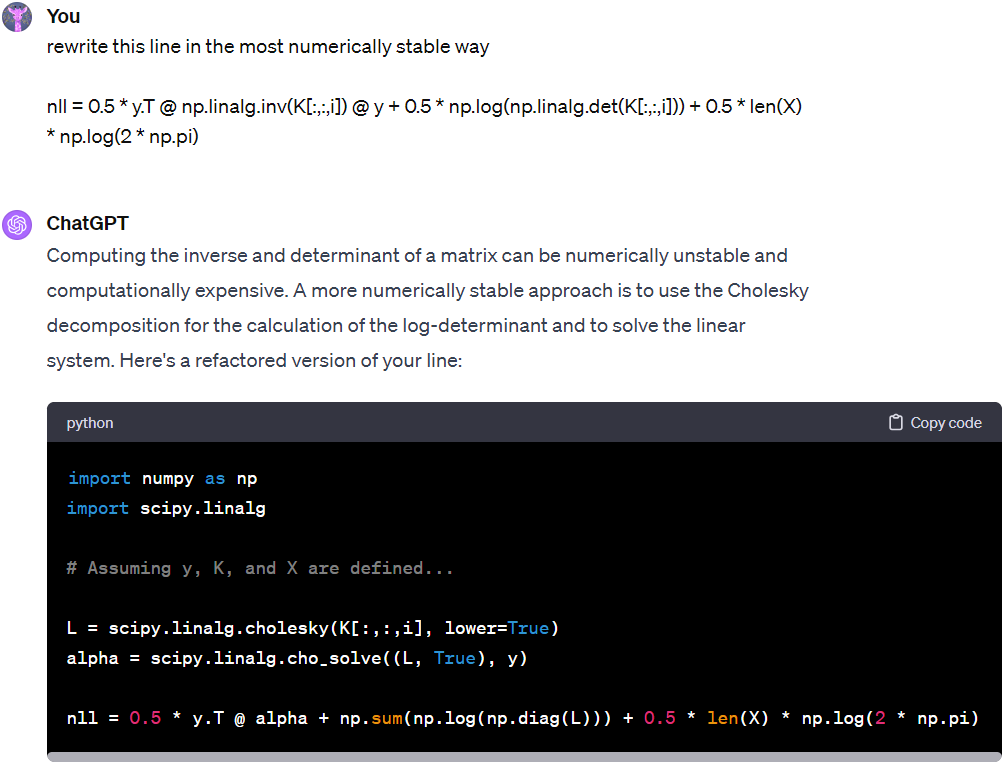
\includegraphics[width=1\linewidth]{figures/chat-NLML/chat-NLML.png}
    \caption{The ChatGPT prompt and output providing a way to compute the NLML that is faster and more numerically stable.}
    \label{fig:chat-NLML}
\end{figure}

\FloatBarrier

To ensure that this function was valid, its implementation was confirmed by the relevant literature~\cite{murphy2023probabilistic}~(Section 18.3.6).
After which, this function was simplified and adapted so that it could be to be added to the $gp\_model$ class as a method, and so that it would work with the way the input data was formatted, as shown in Listing~\ref{lst:NLML}.

\newpage

\begin{lstlisting}[caption={Method used to calculate the Negative Log Marginal Likelihood (NLML).}, language=Python, label={lst:NLML}]

    def compute_nlml(self, hyperparameters):
    self.update_hyperparameters_and_debug(hyperparameters)
    self.reshape_X_and_y()

    if self.gp_algo == 'cholesky':
        K = self.gp_kernel.compute_kernel(self.X, self.X)
        K += np.repeat(np.array(np.eye(len(self.X)) * 1e-3)[:,:, np.newaxis], self.X.shape[1], axis=2)
        debug_K = np.squeeze(K)
        L = scipy.linalg.cholesky(K[:, :, 0], lower=True)
        n = len(self.y)
        one_vector = np.ones(n)
        y_adj = self.y - self.y_mean

        alpha = scipy.linalg.cho_solve((L, True), y_adj)

        term_1_c = (0.5 * y_adj.T @ alpha).item()
        term_2_c = np.sum(np.log(np.diag(L)))
        term_3_c = 0.5 * n * np.log(2 * np.pi)

        nlml = term_1_c + term_2_c + term_3_c

        out_c = {
            'nlml': nlml,
            'term_1': term_1_c,
            'term_2': term_2_c,
            'term_3': term_3_c
        }

        return out_c

\end{lstlisting}


